\NextFile{tuning.html}

\chapter{Printer Calibration} \label{chap:tuning}

To get the best quality prints from your printer, you should invest some time in calibrating your slicing profiles to your printer.  Also, if you have a printer with two extruders, you should calibrate your \glspl{toolhead offset} so as to ensure good alignment in prints which use both extruders.

\NextFile{tuning-slicer-calibration.html}

\section{Slicer Calibration}
\index{Calibration!Slicing profile}

To get top quality prints, you will need to invest some time in calibrating
your \glspl{slicing profile} to suit both your printer and choice of filaments.
Fortunately, the process (presented in Section~\ref{sec:cube}) is simple and straightforward, though it does require a basic understanding of your slicing software.

%The overwhelming majority of users need only perform a basic calibration
%with the ``calibration cube''.  This is presented in Section~\ref{sec:cube}.
%Some users may be interested in also adjusting the JKN ``K'' and ``K2''
%parameters.  However, the default settings found in your printer are likely
%quite good already and not in need of any changes.

\NextFile{tuning-slicer-calibration-filament-diameter.html}

\subsection{Filament Diameter}
\index{Under-extrusion}
\index{Over-extrusion}

The need to measure your filament diameter before preparing a model for
printing \emph{cannot be stressed enough}.  It is important that you have use
of a caliper with which to measure the diameter of your filament.\footnote{A
digital caliper is easiest to use although a dial or vernier caliper will
work just as well.  You will need to produce measurements in units of
millimeters, mm.  Consequently, calipers which directly read in those units
is preferred.  Otherwise, you will need to convert to units of mm.}  Filament
sold as 1.75~mm filament may in fact be 1.68 or 1.85~mm in diameter.  However,
when preparing models for printing, especially large models,
it is critical that the slicing process know the actual diameter of the
filament.  Otherwise too much or too little filament will be extruded, as
the slicer determines the amount of filament needed based upon the
expected volume per millimeter of raw input filament.  If the actual diameter is
larger than expected, too much plastic will be extruded and
``\gls{over-extrusion}'' results.  And, if the diameter is smaller than
expected, too little plastic will be extruded and ``\gls{under-extrusion}''
results.

With a calibrated slicing profile and measured filament diameter, very
smooth top surfaces can be achieved when printing.  The blue tag print of
Figure~\ref{fig:smooth-top} is such an example.

\begin{figure}[!htbp]
  \centering
    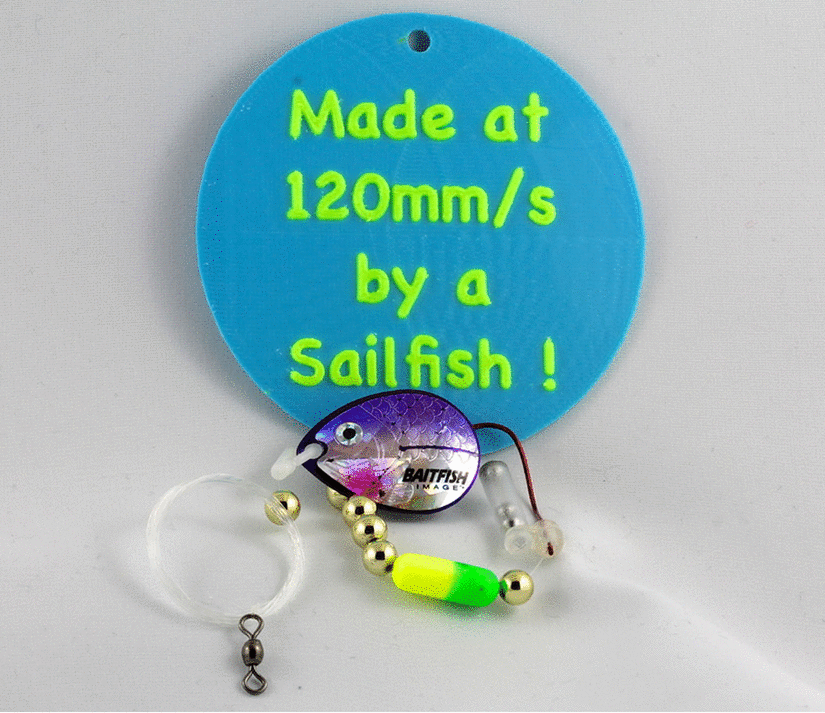
\includegraphics[width=4in]{smooth-top}
    \caption{Smooth surface finish achieved through careful calibration and measurement}
  \label{fig:smooth-top}
\end{figure}

Over and under-extrusion has a cumulative effect: it will not impact small
models nearly as much as it will large models, which may fail to properly print.  Over-extrusion can jam the extruder when the buildup of plastic becomes so much that there is no longer a small gap
between the nozzle and the previously printed layer.  A printed model with
a deficit of plastic --- under-extrusion --- may be too weak to serve
its intended purpose.  Indeed, it may even break apart while being printed
or removed from the build plate.

\NextFile{tuning-slicer-calibration-usb-vs-sd.html}

\subsection{USB vs. SD Card}

If possible, prints should always be run from an SD card.  Printing
over USB introduces additional sources of problems and may result in
prints with small bumps.  \index{Print defects! USB}Accelerated printing runs fast enough that,
if your computer is busy with other tasks, there may occasionally be
small delays introduced to the serial communications.  These delays
can cause the printer to pause for very brief periods of time and
produce small bumps or blemishes --- the result of filament oozing out
of the idle extruder.\footnote{If the computer is not sending commands over USB to the printer, then even features such as deprime (Section \ref{sec:deprime}) and slowdown (Section \ref{sec:slowdown}) will not help prevent the formation of blemishes.}

When calibrating your printer, avoid this additional complication and print
from an SD card.  If you are ever printing over USB and see printing defects
you do not expect, then attempt the same print from an SD card and see
if that leads to an improvement.

\NextFile{tuning-slicer-calibration-know-your-defects.html}

\subsection{Know Your Defects}

Before launching into a discussion of tuning, you should first be
familiar with three particular print defects which, incidentally,
occur with or without accelerated printing and are not unique to Sailfish.  There are other defects as
well, but familiarity with these three is helpful as they may appear on
your calibration boxes.  You may not be used to seeing them when
printing at low speeds (e.g., 40~mm/s), but at higher speeds,
accelerated or otherwise, they will be more likely to manifest.

\subsubsection{Infill telegraphing} \label{sec:telegraphing}
\index{Telegraphing}
\index{Print defects!Telegraphing}

\Gls{infill} \gls{telegraphing}, such as that seen in
Figure~\ref{fig:telegraphing},
often occurs when printing with a single \gls{shell} and under-extruding.
It may also be caused by a hot extruder nozzle dragging over or pushing
into the layer below it, as can occur when over-extruding.  Make sure
that you correctly measured the filament diameter and supplied that value to your
slicer when slicing.  Also, be sure to calibrate your extruder as outlined in
Section~\ref{sec:cube}.

\begin{figure}[!htbp]
  \centering
    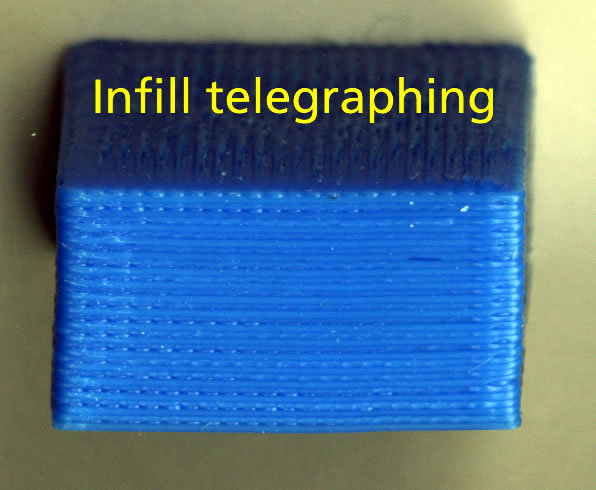
\includegraphics[width=3in]{telegraphing}
    \caption{Infill telegraphing through the print's perimeter}
  \label{fig:telegraphing}
\end{figure}

Any overshoot caused during infill direction changes may also cause this effect, in which case an extra
shell will help hide it. If excess momentum is implicated, then the
same techniques used to reduce corner ringing
(Section~\ref{sec:ringing}), may also be applied here.

A short term fix may be to slice your model with an additional shell or two.

Note that Figure \ref{fig:telegraphing} is an extreme case --- to the point where the
infill itself is visible between some of the perimeter's layers. On
some of the layers where the infill is not directly visible, ripples caused by
it or the nozzle pushing against the inside of the perimeter may still be
visible.

\subsubsection{Ringing} \label{sec:ringing}
\index{Ringing}
\index{Corner ringing}
\index{Print defects!Ringing}

At higher print speeds, when the motion of the build platform or
extruder makes a sudden change in direction, a ringing vibration may
occur.\footnote{In severe cases, there may be actual overshoot caused
by the extruder carriage's momentum carrying it farther than intended.
At issue is that the printer has no feedback mechanism and thus
does not know whether the maximum rates of acceleration and deceleration with which it
has been configured are actually achievable.}  Since
sudden direction changes are often associated with turning a corner in
the print, this effect is often referred to as ``\gls{corner
ringing}''.

\begin{figure}[!htbp]
  \centering
    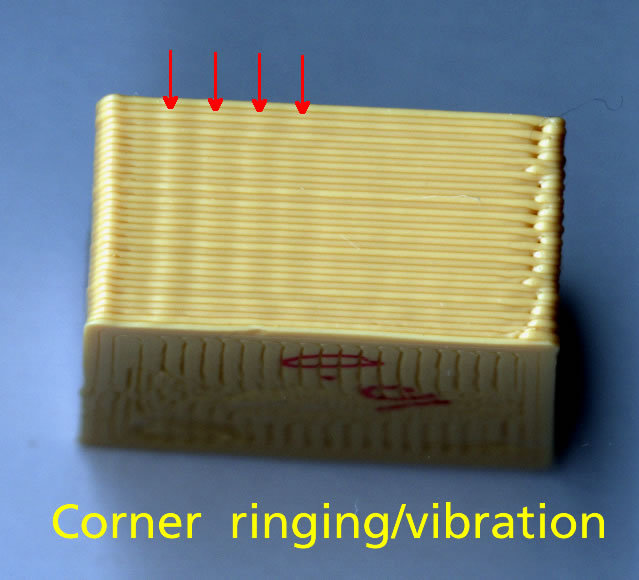
\includegraphics[width=3in]{corner-ringing}
    \caption{Ripples caused by ringing}
  \label{fig:ringing}
\end{figure}

Although quickly dampened, this ringing nonetheless impacts surface
finish, as can be seen in Figure~\ref{fig:ringing}. Ringing is
particularly noticeable on long, flat surfaces and appears as ripples
which rapidly diminish in amplitude. Like infill telegraphing, this
can occur with non-accelerated printing as well as accelerated
printing. The advantage of accelerated printing is that acceleration
can be used to mitigate the issue while still attaining high print
speeds away from corners by lowering the maximum X and Y speed change
values, the maximum X and Y accelerations, or any combination of the
two. For non-accelerated printing, the only recourse is to print the
entire model at slower speeds.

Also note that the mechanics of a given printer may contribute to ringing
effects.  If you are experiencing problems with ringing, then research
postings about ringing in online forums and newsgroups relevant to your
make of printer.  You can also try rotating your model 45\textdegree\ before slicing.

\subsubsection{Stepper clipping} \label{src:clipping}
\index{Stepper clipping}
\index{Print defects!Stepper clipping}

When infill telegraphing and corner ringing are not present, you may
see some very faint rippling along flat faces when you look carefully
in the right lighting and from the right angle.  Figure~\ref{fig:clipping}
shows a print done on a Thing-o-Matic in ABS plastic which illustrates
this effect.

\begin{figure}[!htbp]
  \centering
    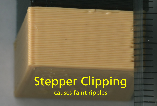
\includegraphics[width=3in]{clipping}
    \caption{Faint ripples caused by stepper clipping}
  \label{fig:clipping}
\end{figure}

This faint rippling may be caused by clipping of the sinusoidal control
signals to the stepper
motors.  Thing-o-Matics and Cupcakes with stepper motors from before
May 2011 are especially vulnerable to this issue.  Unfortunately, later
models suffer as well, as evidenced by the model shown in Figure \ref{fig:clipping} which was
produced on a Thing-o-Matic with post May 2011 stepper motors. Ed
Nisley described and analyzed this in his May 2011 blog posting,
\myhref{http://softsolder.com/2011/05/05/thing-o-matic-mbi-stepper-motor-analysis/}{Thing-o-Matic: MBI Stepper Motor Analysis}, found
at softsolder.com.  At low speeds, this clipping produces a faint
repeating pattern of about 25~Hz. At much higher stepper speeds, the pattern
has a frequency of 50~Hz. Hardware replacement is needed to nearly
eliminate the problem: stepper motors with winding resistances at or
below 2~Ohms, sufficient pull in torque, sufficiently low inductance,
and stepper drivers capable of handling the motors (e.g.,
Pololu).

Significantly slowing down the exterior printing speed may help mitigate
the effects of stepper clipping.  On well-designed and tuned printers,
this is often the one remaining print quality issue.  On suboptimal
or untuned printers, it is still present but hidden by more visible
printing defects.

\NextFile{tuning-slicer-calibration-box.html}

\subsection{Calibration Box} \label{sec:cube}
\index{Calibration!Box|(}

To achieve quality prints, start by ensuring that you can print a decent
calibration ``box'' whose top is nice and flat.  Producing a respectable box
involves calibrating a slicing profile to your printer and choice of
filaments.  So, until you can print a good calibration box, there is little
point in worrying about other printing defects you may be
experiencing.  Here is the step-by-step procedure for
accomplishing this calibration:

\begin{enumerate}

\item Obtain a model for a 10~mm high box which is 20~mm on a side.  ReplicatorG contains as its first example this calibration box:
look under the Examples section of the File menu.  It is the
{\smaller\texttt{20mm\textunderscore Calibration\textunderscore Box.stl}}.
Alternatively, \myhref{http://www.thingiverse.com/thing:2064}{Thing~\#2064} at thingiverse.com contains the calibration box as the download file {\smaller\texttt{20mmbox.stl}}.

\item Use calipers to measure the diameter of the filament with which you will be printing.

\item With the calibration box model in your slicer, slice it at a 0.3~mm
layer height, 100\% infill, and using the diameter of the filament you just
measured.\footnote{If using ReplicatorG with Skeinforge-50,
then do \emph{not} use hexagonal infill.   There is a bug in SF-50's hexagonal
infill which will result in irregular infill; use grid rectangular or line infill instead}  It is critical that you use
100\% infill and that you measure the diameter of your filament and input that
to the slicer.

\item Print the box.

\item Carefully examine the top surface of the box.  While it is easy to
see if the top is convex, you may need to use a
straight edge to gauge how flat or concave the top is.

\begin{enumerate}
\item If it is nice and flat, then you are done!
\item If it is convex, then
too much plastic was extruded and your printer is over-extruding.
Configure your slicing profile to put out slightly less plastic.  How you will do
this depends upon which slicer you use. For ReplicatorG, increase the 
``filament packing density'' in the Dimension plugin.  For MakerBot MakerWare
and Desktop, increase the ``feedstockMultiplier''.  For Simplify3D, reduce the
``extrusion multiplier''.  Only change the value in small increments, such as 0.05.
\item If it is slightly hollow (concave), then too little plastic was
extruded: your printer is under-extruding.  Decrease the filament packing
density (ReplicatorG), decrease the feedstockMultiplier (MakerWare and Desktop),
or increase the extrusion multiplier (Simplify3D).
\end{enumerate}

\item Go back to Step 3, reslicing, reprinting, and re-evaluating the result.
\end{enumerate}

If you happen to have two extruders, it is recommended to do this
calibration once for each extruder.  Then keep distinct slicing
profiles for each extruder: one for the right extruder and another
for the left extruder.

Once you can print a nice calibration box, you are ready to get back
to printing.  Keep in mind that this calibration process
should be repeated for different type of plastics.  At issue is the
differing hardnesses of the plastics used.  The pinch gear in your
printer's extruder feed mechanism bites into the plastic filament.
The depth to which it bites depends upon the hardness of the plastic.
And the deeper the bite, the smaller the effective turning radius of
the gear.  With smaller turning radius, less filament is fed per
rotation of the extruder stepper motor.  This calibration is primarily to address your extruder's handling of these variations in hardness.  For example, ABS is
significantly softer than PLA and so significantly different
adjustments may be needed for ABS versus PLA.  This will, of course,
depend upon the geometry of the pinch gear and how capable it is of
biting into the filament.
\index{Calibration!Box|)}

\NextFile{tuning-dual-extruder-calibration.html}

\section{Dual Extruder Calibration} \label{sec:dual-calib}
\index{Offsets!Toolhead}
\index{Toolhead offsets}
\index{Toolhead offsets!Calibrating|(}
\index{Calibration!Dual extrusion|(}

If your printer has only a single extruder, or if you never use two extruders for the same print, then you can skip this section.

When printing with both extruders, optimal print quality is achieved by precisely calibrating the distance between the two extruder nozzles.  As explained in Section~\ref{sec:toolheadoffsets}, this calibration information is stored as the ``toolhead offsets''.  In this section, a method of determining the toolhead offsets is presented. For every major type of printer, there is a nozzle calibration print in ``ReplicatorG 40 -- Sailfish'', that may be printed as described and then the results supplied to your printer.  Using the results of your print, your printer will then set the correct values for the toolhead offsets.

\begin{enumerate}
\item Before you begin, ensure that you have the latest Replicator G 40 -- Sailfish downloaded from the \myhref{http://www.thingiverse.com/thing:32084}{Sailfish ``Thing'' at Thingiverse}.
\item Launch ReplicatorG and select the correct machine type under the ``Machine Type'' item of the ``Machine'' menu.  Be sure that the machine type name includes ``(Sailfish)'' in it.  Figure~\ref{fig:repg-driver-2} shows The Replicator Dual (Sailfish) selected.

\begin{figure}[!htbp]
  \centering
    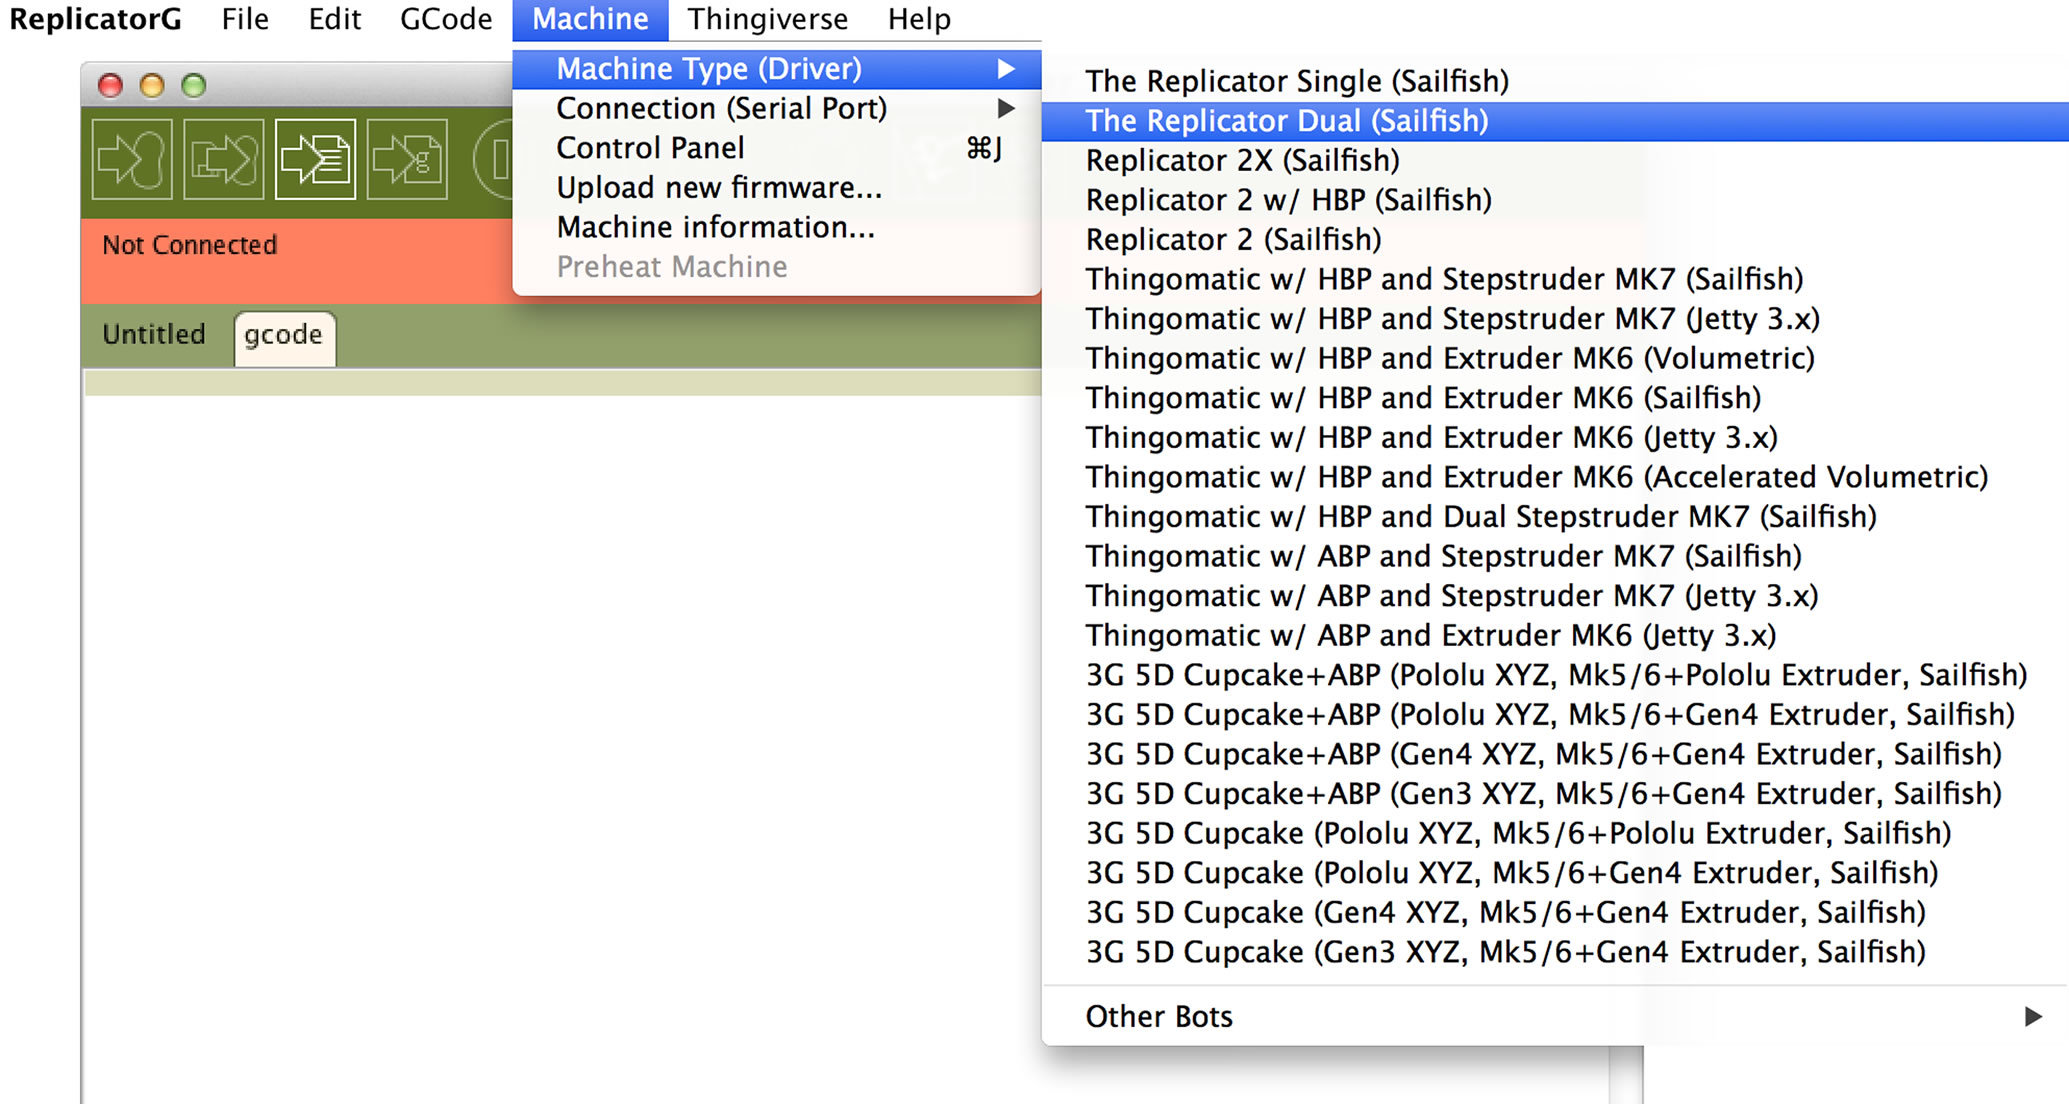
\includegraphics[width=5in]{repg-driver}
    \caption{Machine Type}
  \label{fig:repg-driver-2}
\end{figure}

\item Connect to your printer over USB (see Figure~\ref{fig:repgconnect}), then invoke the \Gls{onboard parameters} window with the ``Onboard Parameters'' item of the ``Machine'' menu.

\begin{figure}[!htbp]
  \centering
    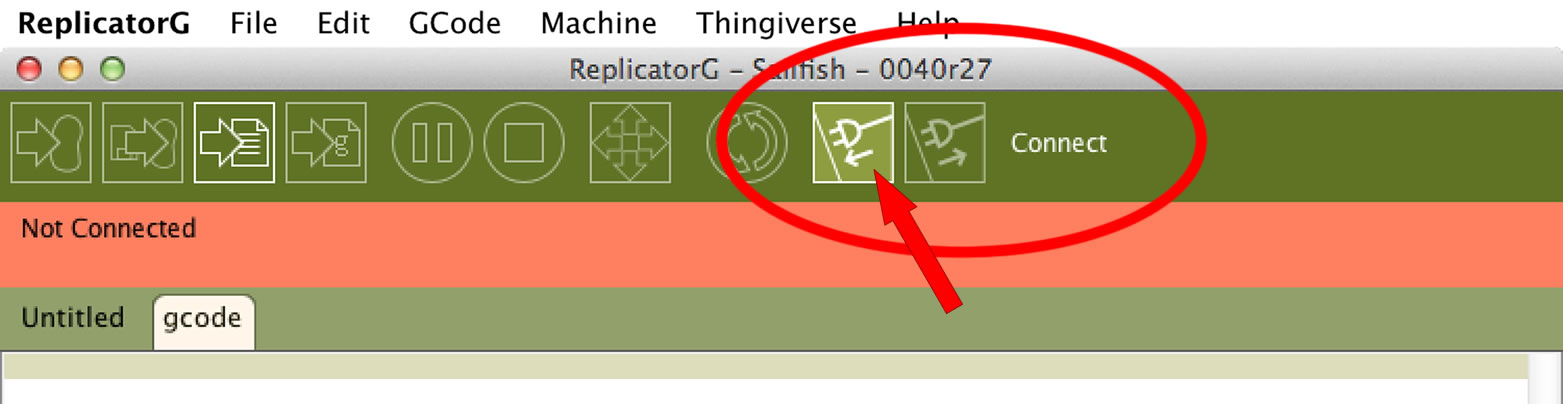
\includegraphics[width=5in]{repg-connect}
    \caption{Connecting to Your Printer}
  \label{fig:repgconnect}
\end{figure}

\item In the ``Homing/VREFs'' tab, set the X and Y toolhead offsets to 0.0~mm.  Be sure to change the toolhead offsets and \emph{not} the home offsets (Figure~\ref{fig:tool-head-settings}).  Make sure to commit the change.  Note that resetting the printer to factory defaults will \emph{not} reset the X and Y toolhead offsets.

\begin{figure}[!htbp]
  \centering
    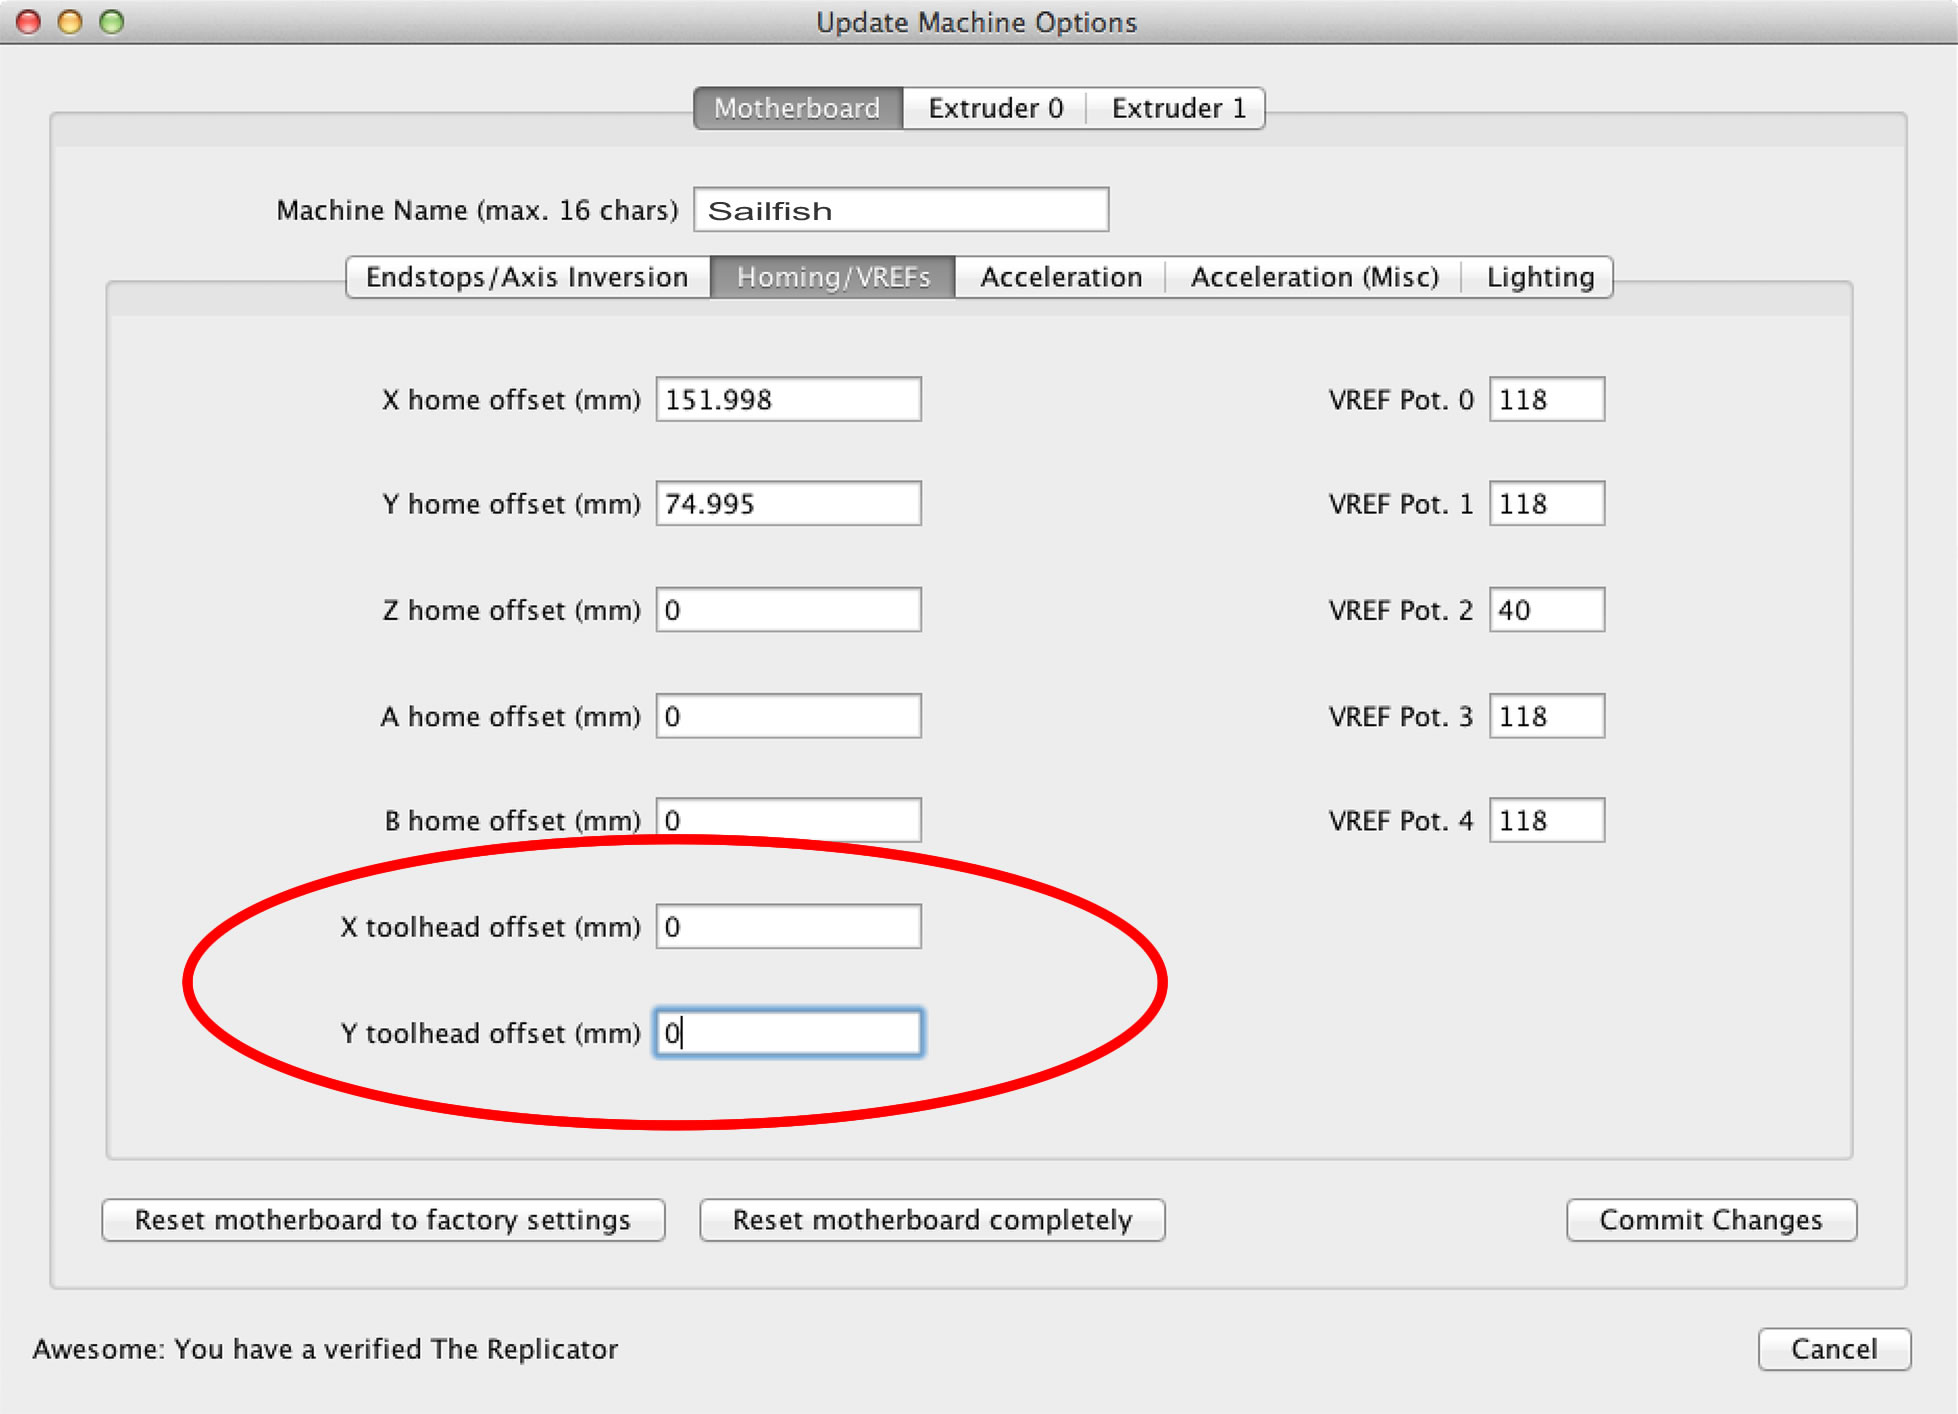
\includegraphics[width=5in]{tool-head-settings}
    \caption{Toolhead Offsets}
  \label{fig:tool-head-settings}
\end{figure}

\item To print the nozzle calibration print go to the ``Scripts'' item of the ``File'' menu, choose your printer type, and then select the ``Dual~Nozzle~Calibration.gcode'' item (Figure~\ref{fig:nozzle-calibration-script}).  Select the Replicator 1 if you do not see your printer type listed.  Note that the name may be an elongated version of this such as ``Flashforge~Creator~Dual~Nozzle~Calibration.gcode''.  Regardless, selecting this will bring up the \gls{gcode} file in ReplicatorG which you should then print to your printer.

\begin{figure}[!htbp]
  \centering
    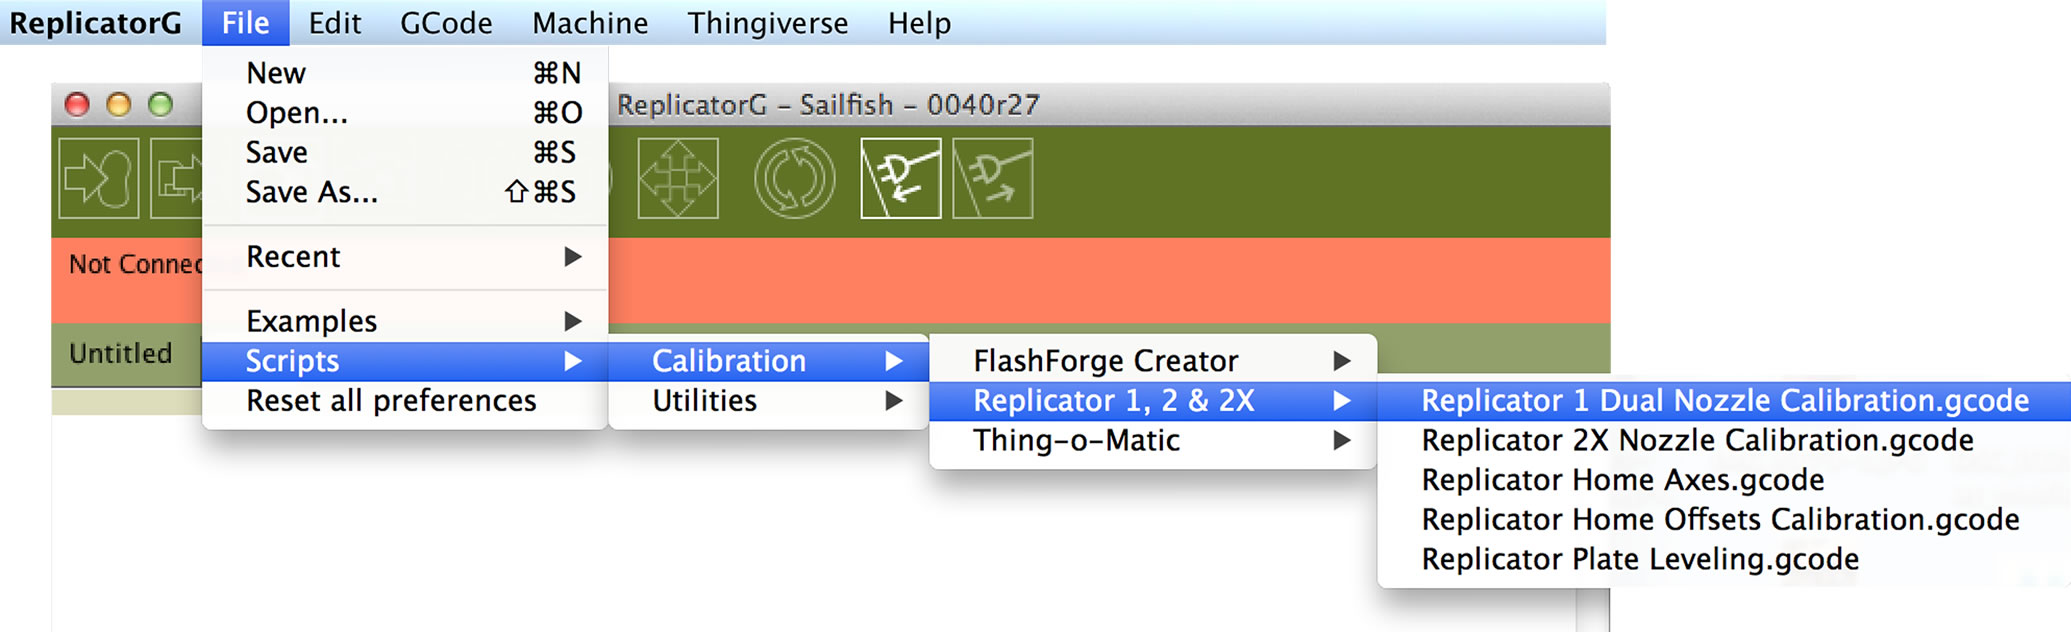
\includegraphics[width=5in]{nozzle-calibration-script}
    \caption{Nozzle Calibration Menu}
  \label{fig:nozzle-calibration-script}
\end{figure}

\item Once the print is finished, you will see a series of horizontal line pairs running vertically up the left side of the build plate (Figure~\ref{fig:nozzle-calibration-print}).  Each pair of lines was printed using both extruders, and is numbered with a value between 1 to 13.  Line 1 is at the front of the plate and should be the longest.  Identify the pair for which each line is vertically the best aligned.  Remember this number.  In the example print of Figure~\ref{fig:nozzle-calibration-print}, either lines 1 or 2 seem to have the best alignment.

\begin{figure}[!htbp]
  \centering
\ifpdf
    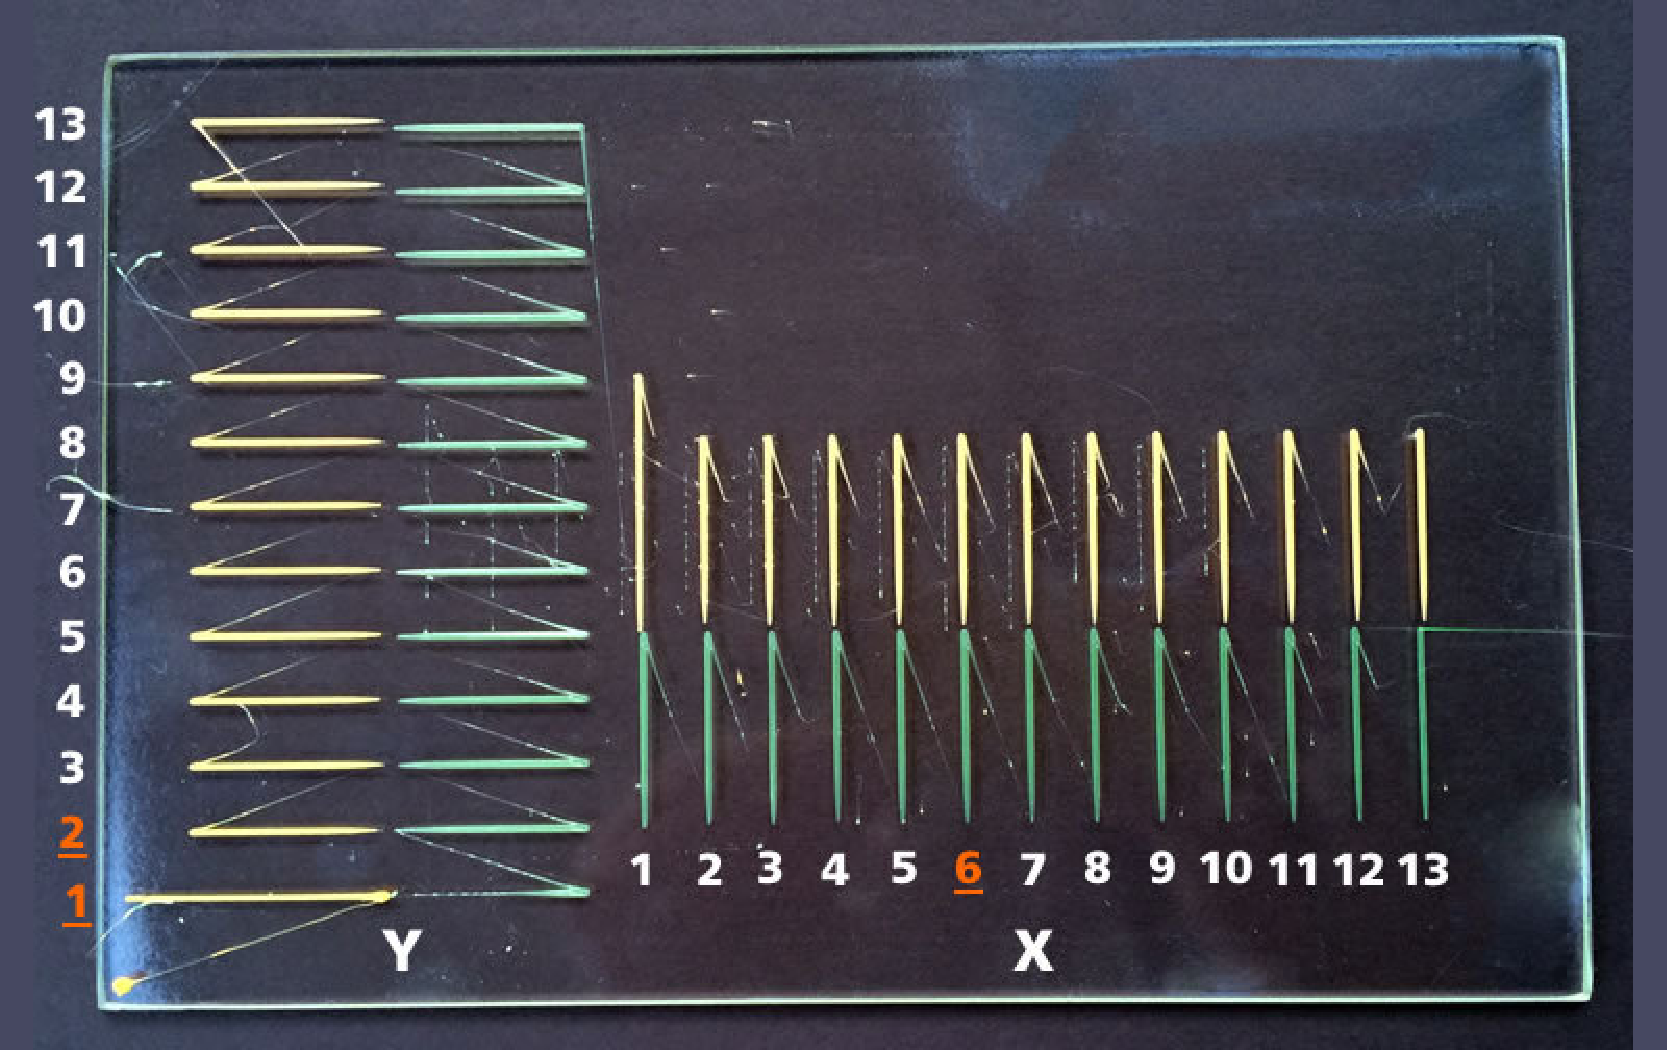
\includegraphics[width=5in]{nozzle-calibration-print}
\else
    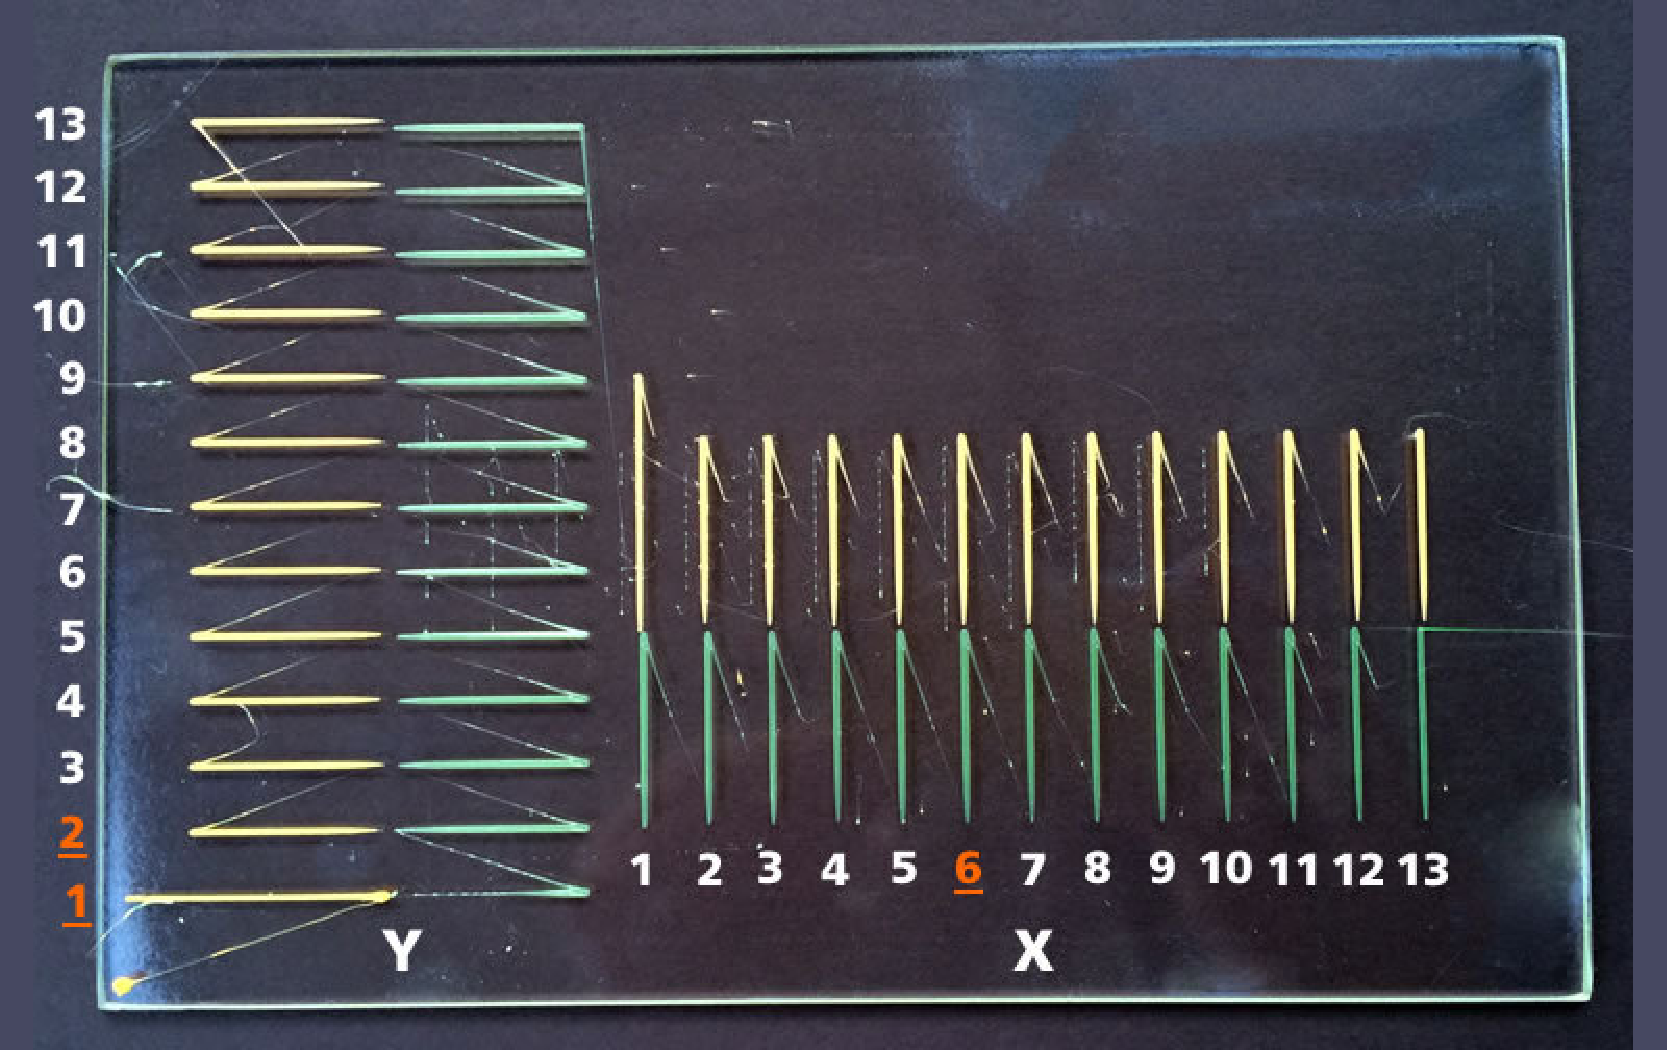
\includegraphics[width=8in]{nozzle-calibration-print}
\fi
    \caption{Nozzle Calibration Print}
  \label{fig:nozzle-calibration-print}
\end{figure}

\item The print will also have a series of vertical line pairs running horizontally across the front of the build plate.  Again, each pair of lines was printed with both extruders, and are numbered 1 to 13.  Line 1 is the leftmost and should also be the longest.  Identify which pair has the best alignment --- which pair has the middle ends closest horizontally.  Remember this number.  In the example print of Figure~\ref{fig:nozzle-calibration-print}, pair 6 appears best aligned.

\item On the printer's LCD screen navigate to the ``Calibrate Nozzles'' item under the ``Utilities'' menu (Section~\ref{sec:calibnozz}).  For the X and Y values, input the numbers you recorded for steps 7 and 6, respectively.  Then select the ``Done'' item on the fourth line of the screen.

\item Your toolhead offsets have now been set.  The values in ReplicatorG's Onboard Preferences will have changed unless you entered 7 for both X and Y, as Line 7 represents the ideal offset of 0.0~mm.  The actual lines are offset by by -0.6~mm, -0.5~mm, ..., 0.0~mm, 0.1~mm, ..., 0.6~mm, creating thirteen offsets total.
\end{enumerate}

Note, however, that, should you revisit the Calibrate Nozzles item on your printer, you will \emph{not} see the X and Y values you entered, as the printer does not save these values but instead uses them to recalibrate.  It is worth mentioning that, after recalibration, these values are no longer correct: if you were to reprint the nozzle calibration print, you should now find that Line 7 is the best match for both X and Y.
\index{Toolhead offsets!Calibrating|)}
\index{Calibration!Dual extrusion|)}

\NextFile{tuning-jkn-advance.html}

\section{JKN Advance K} \label{sec:tuning-k}
\index{JKN Advance!K}
\index{Advance|see{JKN Advance}}

The Jetty-Kubicek-Newman (JKN) Advance parameters address extrusion
issues associated with accelerating and decelerating molten plastic
through the extruder. Left uncorrected, these issues can
result in excess plastic at points of low speed (blobbing) as well as
small bumps (blemishes) and small gaps. In truth, some of these issues
are best addressed by using an ac\-cel\-er\-a\-tion-aware slicer or gcode post-processor. However, at present no such tools exist.

The first of the two JKN Advance parameters, K, addresses an issue
associated with a plastic deficit when accelerating and a plastic
surplus when decelerating. You will find a suitable value for K by
looking at the corners of your calibration boxes printed with
acceleration enabled and at reasonably fast speeds. The fill need
not be solid. Indeed, printing with 20\% infill will also be
informative --- make sure that it still looks good.

\begin{bclogo}[logo=\bcinfo, noborder=true, couleurBarre=yellow]{Important}
Before proceeding and expending time and effort, realize that your printer
ships with reasonably well-tuned JKN parameters.  If you are experiencing
printing defects, adjustment of these parameters will likely not be
satisfactory nor resolve any issues you are attempting to address.  The
following tuning information is more here to satisfy the curiosity of idle, technical minds.
\end{bclogo}

Begin calibrating K by ensuring that acceleration is enabled and
that the JKN Advance K2 parameter is set to 0 (Section \ref{sec:tuning-k2}).
Also, make sure that the maximum X and Y axes acceleration values
are at or below 500~mm/s\textsuperscript{2} so as to minimize overshoot effects.  These values may only be set with ReplicatorG -- Sailfish, MakerWare, or Desktop.  To use the latter two, refer to Section \ref{sec:makerware}.

Print a calibration box (Section~\ref{sec:cube}) with the default K
value of 0.005 (Replicator-style printer) or 0.007 (Thing-o-Matic or
Cupcake). Then print two more boxes, one with K set to 0.0025 and
another at 0.0075 (Replicator-style) or 0.005 and 0.009 (Thing-o-Matic
or Cupcake). It can also be helpful to print a calibration box with K set to 0
for comparison.

What you are looking for is a value of K which helps reduce the amount
of extra plastic at the corners but does not reduce it so much that the
corners become bevelled (i.e., foreshortened) or gaps begin appearing
in the solid surface layers (e.g., the box's top face). As you
decrease K below the optimal value, the top infill will be fine but the
extra plastic at the corners will begin to increase.

Keep in mind that there is no single ``ideal'' value for K. You just want to
get it into the right range.

\begin{figure}[!htbp]
  \centering
    \ifpdf
      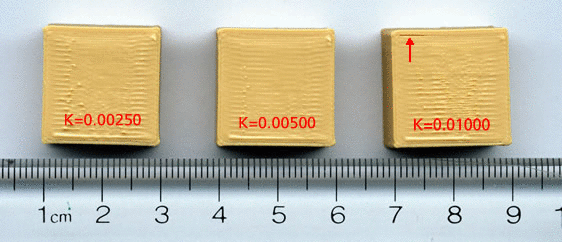
\includegraphics[width=5in]{jkn-advance-k}
    \else
      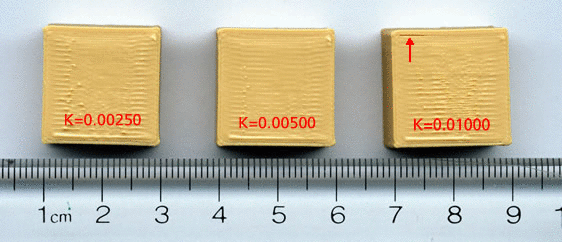
\includegraphics{jkn-advance-k}
    \fi
    \caption{Calibrating JKN Advance K --- calibration boxes printed on a Thing-o-Matic with ABS plastic}
  \label{fig:jkn-advance-k}
\end{figure}

Examine the three calibration boxes shown in Figure~\ref{fig:jkn-advance-k}.  As you can see, the box
on the right with K=0.01000 is showing some gaps, so the value of K is
too large. The middle box with K=0.00500 has a reasonable top surface but
the corners might do with a little less plastic, so K is too small. The leftmost box, K=0.00250 could stand to have a better top surface, again, K is too small. For Thing-o-Matics with an Mk7 extruder, a better value of
K probably exists between 0.00500 and 0.01000.  Note that the firmware's
default value for Thing-o-Matics is 0.00850.  A different default value for
K is used on Replicator-style printers since they use a different extruder and
{\relsize{+1}\textfrac{1}{16}} microstepping --- compared the
Thing-o-Matic's {\relsize{+1}\textfrac{1}{8}}.

\NextFile{tuning-jkn-advance2.html}

\section{JKN Advance K2} \label{sec:tuning-k2}
\index{JKN Advance!K2}

The JKN Advance K2 parameter further corrects for o\-ver-pres\-sur\-i\-za\-tion
in the extruder during the deceleration phase. This is because the
pressurization during the acceleration phase and the depressurization
during the deceleration phase are not symmetrical in effect.

JKN Advance K2 is used to reduce blobbing and splaying in the corners
of boxes and at sharp angles between line segments.

To tune this value, begin by tuning JKN Advance K first as per
Section~\ref{sec:tuning-k}.  When tuning K2, leave K set to the value you
arrived at from that step: do not set K to zero when tuning K2 unless
you found zero to be the best choice for K.

Start by printing a calibration box with K2 set to 0 and 100\%
infill.  Look at the corners: you will see they protrude in the
direction of the filament travel. Increase K2 in units of 0.001 and
check again. Keep increasing JKN Advance K2 in units of 0.001 until
the corners are pulled in as much as possible.

When JKN Advance K2 is set too high, you will begin to see breakup in the top
surface of the box.

Note that the firmware's default value is 0.055 (Replicator-style
printers) and 0.004 (Thing-o-Matic, Cupcake).

\begin{figure}[!htbp]
  \centering
    \ifpdf
      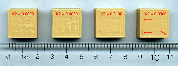
\includegraphics[width=5in]{jkn-advance-k2}
    \else
      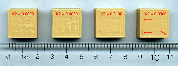
\includegraphics{jkn-advance-k2}
    \fi
    \caption{Calibrating JKN Advance K2 --- calibration boxes printed on a Thing-o-Matic with ABS plastic}
  \label{fig:jkn-advance-k2}
\end{figure}

All four boxes shown in Figure~\ref{fig:jkn-advance-k2} have
K=0.00850, the default value for K on a Thing-o-Matic. The
leftmost box, K2=0.0000, shows the corners when K2 is not
applied. The second box with K2=0.0050 shows a little improvement
with the two upper corners not projecting quite as much. The third
box with K2=0.0100 is just beginning to show some of the infill
plastic pulling away from the perimeter loops. This is quite
noticeable for the final box with K2=0.0300. A good value of K2 is
likely to be found between K2=0.0050 and K2=0.0100. Note that the
differences will be more noticeable to you when you have actual boxes
in your hands which you can look at from all angles. The pictures here
do not fully illustrate the effect of K2 on the prints.
